An \glsdesc{acr:oqe} \gls{seismicsourceinputmodel} contains a list of sources
belonging to a finite set of possible typologies. Each source type is defined
by a set of parameters - called source data - which are used to specify the
source geometry and the properties of seismicity occurrence.

Currently the \glsdesc{acr:oqe} supports the following source types:

\begin{itemize}

    \item Sources for modelling distributed seismicity:

    \begin{itemize}

        \item \Gls{pointsource} - The elemental source type used to model
        distributed seismicity. Grid and area sources (described below) are
        different containers of point sources.

        \item \Gls{areasource} - So far, the most frequently adopted source
        type in national and regional PSHA models.

        \item \Gls{gridsource} - A replacement for area sources admitting
        spatially variable seismicity occurrence properties.

    \end{itemize}

    \item Fault sources with floating ruptures:

    \begin{itemize}

        \item \Gls{simplefaultsource} - The simplest fault model in the
        \glsdesc{acr:oqe}. This source is habitually used to describe shallow
        seismogenic faults.

        \item \Gls{complexfaultsource} - Often used to model subduction
        interface sources with a complex geometry.

    \end{itemize}

    \item Fault sources with ruptures always covering the entire fault surface:

    \begin{itemize}

        \item \Gls{charfaultsource} - A typology of source where ruptures
        always fill the entire fault surface.
        
        \item \Gls{nonparametricsource} - A typology of source representing
        a collection of ruptures, each with their associated probabilities
        of 0, 1, 2 ... occurrences in the investigation time

    \end{itemize}

    \item Sources for representing individual earthquake ruptures
    
    \begin{itemize}
        \item Planar fault rupture - an individual fault rupture represented as a single rectangular plane
        \item Multi-planar fault rupture - an individual rupture represented as a collection of rectangular planes
        \item Simple fault rupture - an individual fault rupture represented as a simple fault surface
        \item Complex fault rupture - an individual fault rupture represented as a complex fault surface
    \end{itemize}

\end{itemize}

The \glsdesc{acr:oqe} contains some basic assumptions for the definition of
these source typologies:

\begin{itemize}

    \item In the case of area and fault sources, the seismicity is
    homogeneously distributed over the source;

    \item Seismicity temporal occurrence follows a Poissonian model.

\end{itemize}

The above sets of sources may be referred to as ``parametric'' sources, that
is to say that the generation of the \Gls{earthquakeruptureforecast} is done
by the OpenQuake engine based on the parameters of the sources set by the
user. In some cases, particularly if the user wishes for the temporal
occurrence model to be non-Poissonian (such as the lognormal or Brownian
Passage Time models) a different type of behaviour is needed. For this
OpenQuake-engine supports a \Gls{nonparametricsource} in which the
\Gls{earthquakeruptureforecast} is provided explicitly by the user as a set of
ruptures and their corresponding probabilities of occurrence.

\subsection{Source typologies for modelling distributed seismicity}
\subsubsection{Point sources}
\label{subsubsec:point_sources}
\index{Source type!point}
\index{Point source|see{Source type}}

\begin{figure}[!ht]
\centering
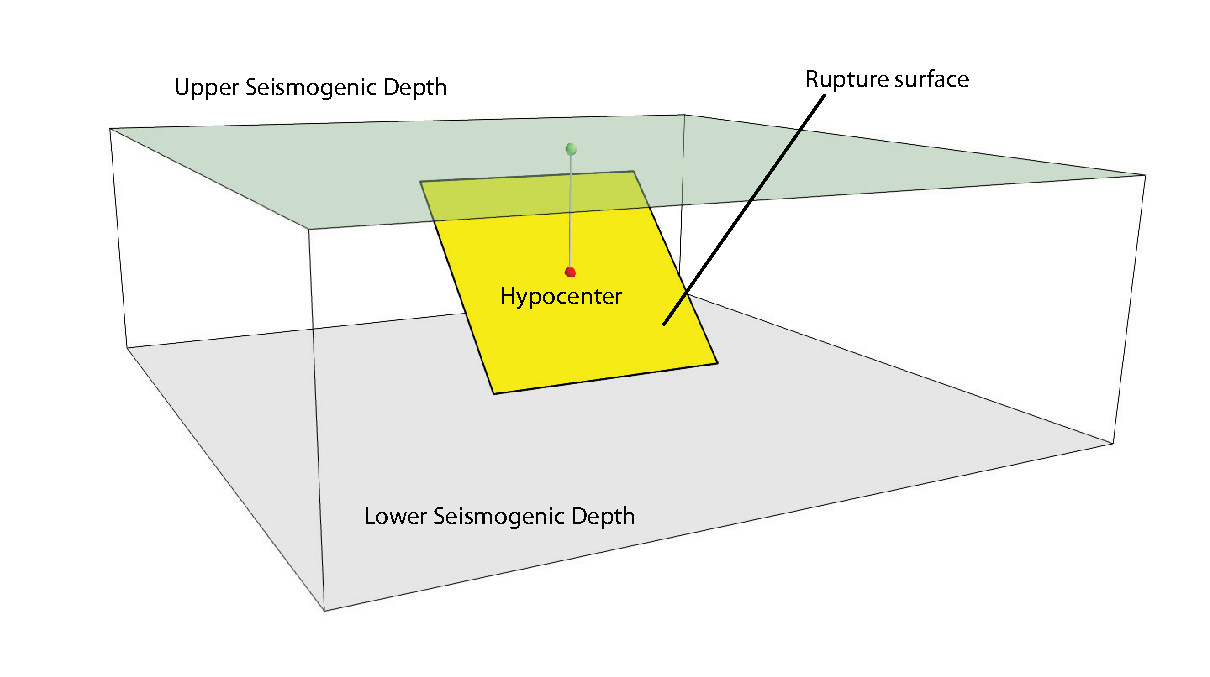
\includegraphics[width=10cm]{figures/hazard/single_rupture.pdf}
\caption{Single rupture}
\label{fig:single_rupture}
\end{figure}

The point source is the elemental source type adopted in the OpenQuake-engine
for modelling distributed seismicity. The \glsdesc{acr:oqe} always performs
calculations considering finite ruptures, even in the case of point sources.

These are the basic assumptions used to generate ruptures with point sources:

\begin{itemize}

    \item Ruptures have a rectangular shape

    \item Rupture hypocenter is located in the middle of the rupture

    \item Ruptures are limited at the top and at the bottom by two planes
    parallel to the sea level and placed at two characteristic
    depths named upper and lower seismogenic depths, respectively (see
    Figure~\ref{fig:single_rupture})

\end{itemize}

\paragraph{Source data}

For the definition of a point source the following parameters are required
(Figure~\ref{fig:single_rupture} shows some of the parameters described
below, together with an example of the surface of a generated rupture):

\begin{itemize}

    \item The coordinates of the point (i.e. longitude and latitude) [decimal
    degrees]

    \item The upper and lower seismogenic depths [km]

    \item One \gls{mfd}

    \item One magnitude-scaling relationship

    \item The rupture aspect ratio

    \item A distribution of nodal planes i.e. one (or several) instances
    of the following set of parameters:

    \begin{itemize}
        \item \gls{strike} [degrees]
        \item \gls{dip} [degrees]
        \item \gls{rake} [degrees]
    \end{itemize}

\item A magnitude independent depth distribution of hypocenters [km].

\end{itemize}

Figure~\ref{fig:point_source_multiple_ruptures} shows ruptures generated by a
point source for a range of magnitudes. Each rupture is centered on the
single hypocentral position admitted by this point source. Ruptures are
created by conserving the area computed using the specified magnitude-area
scaling relatioship and the corresponding value of magnitude.

\begin{figure}[ht!]
\centering
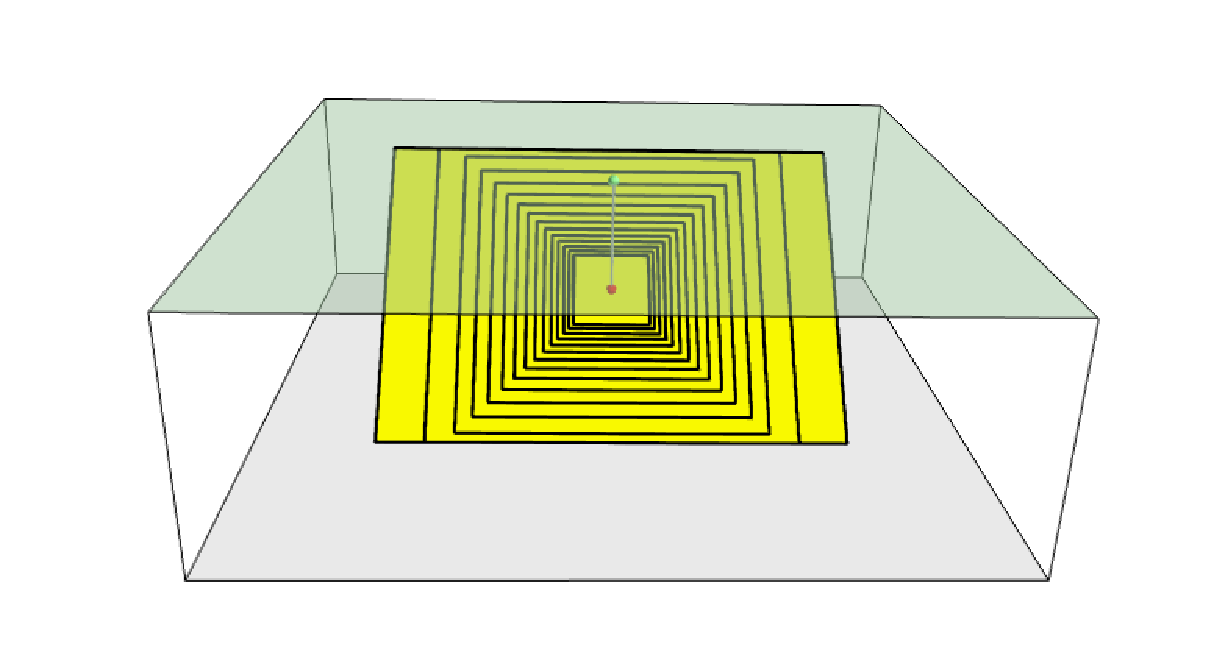
\includegraphics[width=10cm]{figures/hazard/point_source_multiple_ruptures.pdf}
\caption{Point source with multiple ruptures. Note the change in the aspect
ratio once the rupture width fills the entire seismogenic layer.}
\label{fig:point_source_multiple_ruptures}
\end{figure}

Below we provide the excerpt of an .xml file used to describe the properties of a point source. Note that in this example, ruptures occur on two possible nodal planes and two hypocentral depths. Figure~\ref{fig:point_source_ruptures} shows the ruptures generated by the point source.

\begin{listing}[htbp]
  \inputminted[firstline=1,firstnumber=1,fontsize=\footnotesize,frame=single,linenos,bgcolor=lightgray]{xml}{oqum/hazard/verbatim/input_point_source.xml}
  \caption{Example point source}
  \label{page:point_source_nrml}
\end{listing}

%The red part shows the the parameters used to describe the geometry of the point source, the blue part is the description of the magnitude-frequency distribution, the green text shows the nodal plane distribution and the text in magenta illustrates the hypocentral depth distribution.

%The text in black describes the parameters needed to generate the ruptures such as the \gls{msr} and the aspect ratio.



\begin{figure}[!ht]
\centering
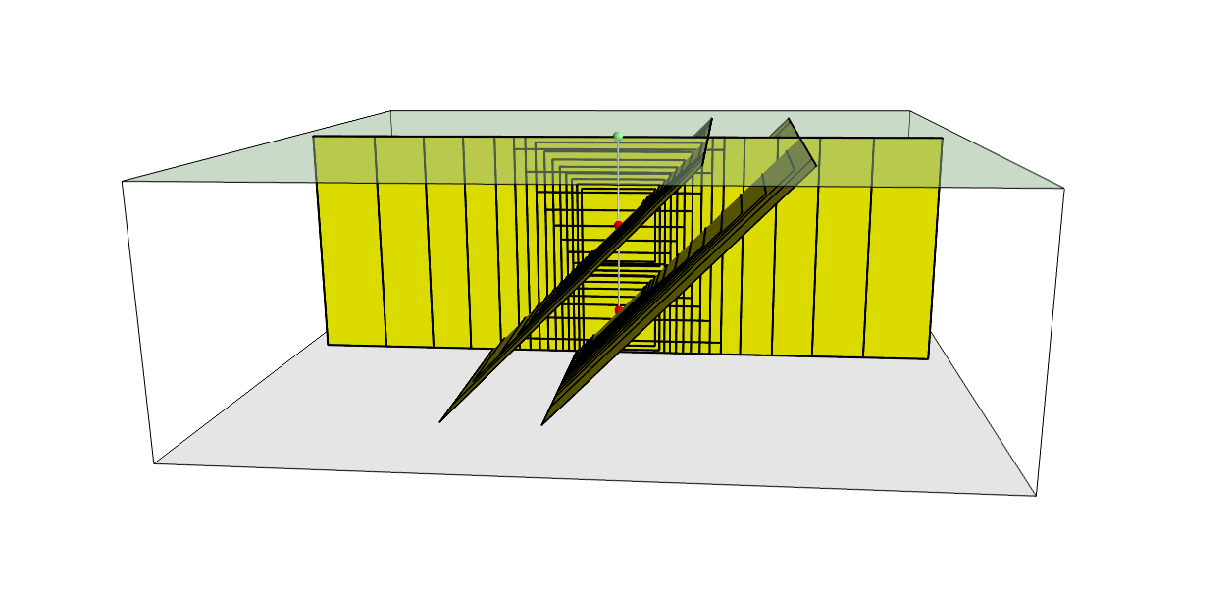
\includegraphics[width=10cm]{figures/hazard/pointsrc_2strike_2hypodep.pdf}
\caption{Ruptures produced by the source created using the information 
in the example .xml file described on page~\pageref{page:point_source_nrml}.}
\label{fig:point_source_ruptures}
\end{figure}

\subsubsection{Grid sources}
\label{subsubsec:grid_sources}
\index{Source type!grid}
\index{Grid source|see{Source type}}

A \gls{gridsource} is simply a collection of point sources distributed over a regular grid (usually equally spaced in longitude and latitude). In \gls{psha} a grid source can be considered a model alternative to area
sources, since they both model distributed seismicity. Grid sources are generally used to reproduce more faithfully the spatial pattern of seismicity depicted by the earthquakes occurred in the past; in
some models (e.g. \citet{petersen2008}) only events of low and intermediate magnitudes are considered. They are frequently, though not always, computed using seismicity smoothing algorithms \citep[][amongst many others]{frankel1995,woo1996}.

The use of smoothing algorithms to produce grid sources brings some
advantages compared to area sources, since (1) it removes most of the
unavoidable degree of subjectivity due to the definition of the geometries of the area sources and (2) it produces a spatial pattern of seismicity that is usually closer to what observed in the reality. Nevertheless, in many cases smoothing algorithms require an a-priori definition of some setup parameters that expose the calculation to a certain degree of partiality.

Grid sources are modeled in \gls{acr:oqe} simply as a set of point sources; in other words, a grid source is just a long list of point sources specified as described in the previous section (see page
\pageref{subsubsec:point_sources}).

\subsubsection{Area sources}
\label{subsubsec:area_sources}
\index{Source type!area}
\index{Area source|see{Source type}}

Area sources are usually adopted to describe the seismicity occurring over wide areas where the identification and characterization - i.e. the
unambiguous definition of position, geometry and seismicity occurrence
parameters - of single fault structures is difficult.

From a computation standpoint, area sources are comparable to grid sources since they are both represented in the engine by a list of point sources.

The \gls{acr:oqe} using the source data parameters (see below) creates an
equally spaced in distance grid of point sources where each point has the same seismicity occurrence properties (i.e. rate of events generated).

Below we provide a brief description of the parameters necessary to completely describe an area source.

\paragraph{Source data}

\begin{itemize}

    \item A polygon defining the external border of the area (i.e. a list of
    Longitude-Latitude [degrees] tuples) The current version of the OQ-engine doesn't
    support the definition of internal borders.

    \item The upper and lower seismogenic depths [km]

    \item One \gls{mfd}

    \item One \gls{msr}

    \item The rupture aspect ratio

    \item A distribution of nodal planes i.e. one (or several) instances of
    the following set of parameters

    \begin{itemize}
        \item \gls{strike} [degrees]
        \item \gls{dip} [degrees]
        \item \gls{rake} [degrees]
    \end{itemize}

    \item A magnitude independent depth distribution of hypocenters [km].

\end{itemize}

Below we provide the excerpt of an .xml file used to describe the properties of an area source. The ruptures generated by the area source described in the example are controlled by two nodal planes and have hypocenters at localized at two distinct depths.

\begin{listing}[htbp]
  \inputminted[firstline=1,firstnumber=1,fontsize=\footnotesize,frame=single,linenos,bgcolor=lightgray]{xml}{oqum/hazard/verbatim/input_area_source.xml}
  \caption{Example area source}
  \label{lst:area_source}
\end{listing}

%The red text describes the parameters used to describe the geometry of the area source; the blue part is the description of the magnitude-frequency distribution; the green text displays the nodal plane distribution; and the text in magenta illustrates the hypocentral depth distribution.

%The text in gray describes the parameters required to generate the ruptures such as the \gls{msr} and the aspect ratio.



\subsection{Fault sources with floating ruptures}
Fault sources in the \gls{acr:oqe} are classified according to the method
adopted to distribute ruptures over the fault surface. Two options are
currently supported:

\begin{itemize}

    \item With the first option, ruptures with a surface lower than the
    whole fault surface are floated so as to cover as much as possible
    homogeneously the fault surface. This model is compatible with all the
    supported magnitude-frequency distributions.

    \item With the second option, ruptures always fill the entire fault
    surface. This model is compatible with magnitude-frequency
    distributions similar to a characteristic model (\`{a} la
    \cite{schwartz1984}).

\end{itemize}

In this subsection we discuss the different fault source types that
support floating ruptures. In the next subsection we will illustrate the fault
typology available to model a characteristic rupturing behaviour.



\subsubsection{Simple faults}
\label{desc_simple_fault}
\index{Source type!fault!simple geometry}
\index{Simple fault|see{Source type}}

Simple Faults are the most common source type used to model shallow faults;
the ``simple'' adjective relates to the geometry description of the source
which is obtained by projecting the fault trace (i.e. a polyline) along a
characteristic dip direction.

The parameters used to create an instance of this source type are described
in the following paragraph.

\paragraph{Source data}

\begin{itemize}

    \item A horizontal \gls{faulttrace} (usually a polyline). It is a list of
    longitude-latitude tuples [degrees].

    \item A \gls{frequencymagnitudedistribution}

    \item A \gls{msr}

    \item A representative value of the dip angle (specified following
    the Aki-Richards convention; see \citet{aki2002}) [degrees]

    \item Rake angle (specified following the Aki-Richards convention;
    see \citet{aki2002}) [degrees]

    \item Upper and lower depth values limiting the seismogenic interval [km]

\end{itemize}

For near-fault probabilistic seismic hazard analysis, two additional
parameters are needed for characterising seismic sources:

\begin{itemize}

    \item A hypocentre list. It is a list of the possible hypocentral
    positions, and the corresponding weights, e.g., alongStrike="0.25"
    downDip="0.25" weight="0.25". Each hypocentral position is defined in
    relative terms using as a reference the upper left corner of the rupture
    and by specifying the fraction of rupture length and rupture width.

    \item A slip list. It is a list of the possible rupture slip directions
    [degrees], and their corresponding weights. The angle describing each slip
    direction is measured counterclockwise using the fault strike direction as
    reference.

\end{itemize}

In near-fault PSHA calculations, the hypocentre list and the slip list are
mandatory. The weights in each list must always sum to one. The available GMPE
which currently supports the near-fault directivity PSHA calculation in OQ-
engine is the ChiouYoungs2014NearFaultEffect GMPE developed  by
\citet{chiou2014update} (associated with an \texttt{Active Shallow Crust}
tectonic region type).

We provide two examples of simple fault source files. The first is an
excerpt of an xml file used to describe the properties of a simple fault
source and the second example shows the excerpt of an xml file used to
describe the properties of a simple fault source that can be used to perform a PSHA calculation taking into account directivity effects.

\begin{listing}[htbp]
  \inputminted[firstline=1,firstnumber=1,fontsize=\footnotesize,frame=single,linenos,bgcolor=lightgray]{xml}{oqum/hazard/verbatim/input_simple_fault.xml}
  \caption{Example simple fault}
  \label{lst:example_simple_fault}
\end{listing}
%\begin{Verbatim}[frame=single, commandchars=\\\{\}, fontsize=\footnotesize,
numbers=left, numbersep=2pt]
<areaSource id="1" name="Quito" tectonicRegion="Active Shallow Crust">
    \textcolor{red}{<areaGeometry>}
        \textcolor{red}{<gml:Polygon>}
            \textcolor{red}{<gml:exterior>}
                \textcolor{red}{<gml:LinearRing>}
                    \textcolor{red}{<gml:posList>}
                    \textcolor{red}{-122.5 37.5}
                    \textcolor{red}{-121.5 37.5}
                    \textcolor{red}{-121.5 38.5}
                    \textcolor{red}{-122.5 38.5}
                    \textcolor{red}{</gml:posList>}
                    \textcolor{red}{</gml:LinearRing>}
            \textcolor{red}{</gml:exterior>}
        \textcolor{red}{</gml:Polygon>}
        \textcolor{red}{<upperSeismoDepth>0.0</upperSeismoDepth>}
        \textcolor{red}{<lowerSeismoDepth>10.0</lowerSeismoDepth>}
        \textcolor{red}{</areaGeometry>}
    \textcolor{gray}{<magScaleRel>PeerMSR</magScaleRel>}
    \textcolor{gray}{<ruptAspectRatio>1.5</ruptAspectRatio>}
    \textcolor{blue}{<incrementalMFD minMag="6.55" binWidth="0.1">}
        \textcolor{blue}{<occurRates>0.0010614989 8.8291627E-4 7.3437777E-4 6.108288E-4}
            \textcolor{blue}{5.080653E-4</occurRates>}
    \textcolor{blue}{</incrementalMFD>}
    \textcolor{green}{<nodalPlaneDist>}
        \textcolor{green}{<nodalPlane probability="0.3" strike="0.0" dip="90.0" rake="0.0"/>}
        \textcolor{green}{<nodalPlane probability="0.7" strike="90.0" dip="45.0" rake="90.0"/>}
    \textcolor{green}{</nodalPlaneDist>}
    \textcolor{magenta}{<hypoDepthDist>}
        \textcolor{magenta}{<hypoDepth probability="0.5" depth="4.0" />}
        \textcolor{magenta}{<hypoDepth probability="0.5" depth="8.0" />}
    \textcolor{magenta}{</hypoDepthDist>}
</areaSource>
\end{Verbatim}
%\label{example_incremental_mfd}

%Below is an excerpt of a simple fault source xml file for near-fault directivity PSHA calculations:

%\begin{listing}[htbp]
\inputminted[firstline=1,firstnumber=1,fontsize=\footnotesize,frame=single,linenos,bgcolor=lightgray]{xml}{oqum/hazard/verbatim/input_simple_fault_directivity.xml}
\captionof{listing}{Example simple fault with added information to model directivity\label{lst:example_simple_fault_directivity}}

%\end{listing}

%\begin{Verbatim}[frame=single, commandchars=\\\{\}, fontsize=\footnotesize,
    numbers=left, numbersep=2pt]
<simpleFaultSource id="1" name="Mount Diablo Thrust"
        tectonicRegion="Active Shallow Crust">
    \textcolor{red}{<simpleFaultGeometry>}
        \textcolor{red}{<gml:LineString>}
            \textcolor{red}{<gml:posList>}
                \textcolor{red}{-121.82290 37.73010}
                \textcolor{red}{-122.03880 37.87710}
            \textcolor{red}{</gml:posList>}
        \textcolor{red}{</gml:LineString>}
        \textcolor{red}{<dip>45.0</dip>}
        \textcolor{red}{<upperSeismoDepth>10.0</upperSeismoDepth>}
        \textcolor{red}{<lowerSeismoDepth>20.0</lowerSeismoDepth>}
    \textcolor{red}{</simpleFaultGeometry>}
    \textcolor{gray}{<magScaleRel>WC1994</magScaleRel>}
    \textcolor{gray}{<ruptAspectRatio>1.5</ruptAspectRatio>}
    \textcolor{blue}{<incrementalMFD minMag="5.0" binWidth="0.1">}
        \textcolor{blue}{<occurRates>0.0010614989 8.8291627E-4 7.3437777E-4 6.108288E-4 }
                \textcolor{blue}{5.080653E-4</occurRates>}
    \textcolor{blue}{</incrementalMFD>}
    \textcolor{green}{<rake>30.0</rake>}
    \textcolor{gray}{<hypoList>}
        \textcolor{gray}{<hypo alongStrike="0.25" downDip="0.25" weight="0.25"/>}
        \textcolor{gray}{<hypo alongStrike="0.25" downDip="0.75" weight="0.25"/>}
        \textcolor{gray}{<hypo alongStrike="0.75" downDip="0.25" weight="0.25"/>}
        \textcolor{gray}{<hypo alongStrike="0.75" downDip="0.75" weight="0.25"/>}
    \textcolor{gray}{</hypoList>}
    \textcolor{gray}{<slipList>}
        \textcolor{gray}{<slip weight="0.333"> 0.0 </slip>}
        \textcolor{gray}{<slip weight="0.333"> 45.0 </slip>}
        \textcolor{gray}{<slip weight="0.334"> 90.0 </slip>}
    \textcolor{gray}{</slipList>}
</simpleFaultSource>
\end{Verbatim}

%As with the previous examples, the red text highlights the parameters used to specify the source geometry, the parameters in green describe the rupture mechanism, the text in blue describes the magnitude-frequency distribution and the gray text describes the rupture properties.



\subsubsection{Complex faults}
\label{desc_complex_fault}
\index{Source type!fault!complex geometry}
\index{Complex fault|see{Source type}}

A complex fault differs from simple fault just by the way the geometry of the
fault surface is defined and the fault surface is later created. The input
parameters used to describe complex faults are, for the most part, the same
used to describe the simple fault typology.

In the case of complex faults, the dip angle is not requested while the fault
trace is substituted by two fault edges limiting the top and bottom of the fault
surface. Additional curves lying over the fault surface can be specified to
complement and refine the description of the fault surface geometry.
Unlike the simple fault these edges are not required to be horizontal
and may vary in elevation, i.e. the upper edge may represent the intersection 
between the exposed fault trace and the topographic surface, where positive values
indicate below sea level, and negative values indicate above sea level.

Usually, we use complex faults to model intraplate megathrust faults such as
the big subduction structures active in the Pacific (Sumatra, South America,
Japan) but this source typology can be used also to create - for example -
listric fault sources with a realistic geometry.

\inputminted[firstline=1,firstnumber=1,fontsize=\footnotesize,frame=single,linenos,bgcolor=lightgray]{xml}{oqum/hazard/verbatim/input_complex_fault.xml}
\captionof{listing}{Example complex fault \label{lst:example_complex_fault}}

%\begin{Verbatim}[frame=single, commandchars=\\\{\}, fontsize=\footnotesize,
    numbers=left, numbersep=2pt]
<complexFaultSource id="1" name="Cascadia Megathrust"
        tectonicRegion="Subduction Interface">
\textcolor{red}{    <complexFaultGeometry>}
\textcolor{red}{        <faultTopEdge>}
\textcolor{red}{            <gml:LineString>}
\textcolor{red}{                <gml:posList>}
\textcolor{red}{                    -124.704  40.363  0.5493260E+01}
\textcolor{red}{                    -124.977  41.214  0.4988560E+01}
\textcolor{red}{                    -125.140  42.096  0.4897340E+01}
\textcolor{red}{                </gml:posList>}
\textcolor{red}{            </gml:LineString>}
\textcolor{red}{        </faultTopEdge>}
\textcolor{red}{        <intermediateEdge>}
\textcolor{red}{            <gml:LineString>}
\textcolor{red}{                <gml:posList>}
\textcolor{red}{                    -124.704  40.363  0.5593260E+01}
\textcolor{red}{                    -124.977  41.214  0.5088560E+01}
\textcolor{red}{                    -125.140  42.096  0.4997340E+01}
\textcolor{red}{                </gml:posList>}
\textcolor{red}{            </gml:LineString>}
\textcolor{red}{        </intermediateEdge>}
\textcolor{red}{        <intermediateEdge>}
\textcolor{red}{            <gml:LineString>}
\textcolor{red}{                <gml:posList>}
\textcolor{red}{                    -124.704  40.363  0.5693260E+01}
\textcolor{red}{                    -124.977  41.214  0.5188560E+01}
\textcolor{red}{                    -125.140  42.096  0.5097340E+01}
\textcolor{red}{                </gml:posList>}
\textcolor{red}{            </gml:LineString>}
\textcolor{red}{        </intermediateEdge>}
\textcolor{red}{        <faultBottomEdge>}
\textcolor{red}{            <gml:LineString>}
\textcolor{red}{                <gml:posList>}
\textcolor{red}{                    -123.829  40.347  0.2038490E+02}
\textcolor{red}{                    -124.137  41.218  0.1741390E+02}
\textcolor{red}{                    -124.252  42.115  0.1752740E+02}
\textcolor{red}{                </gml:posList>}
\textcolor{red}{            </gml:LineString>}
\textcolor{red}{        </faultBottomEdge>}
\textcolor{red}{    </complexFaultGeometry>}
    \textcolor{gray}{<magScaleRel>WC1994</magScaleRel>}
    \textcolor{gray}{<ruptAspectRatio>1.5</ruptAspectRatio>}
\textcolor{blue}{   <truncGutenbergRichterMFD aValue="-3.5" bValue="1.0" minMag="5.0" }
\textcolor{blue}{           maxMag="6.5" />}
\textcolor{green}{   <rake>30.0</rake>}
</complexFaultSource>
\end{Verbatim}

As with the previous examples, the red text highlights the parameters used to
specify the source geometry, the parameters in green describe the rupture
mechanism, the text in blue describes the magnitude-frequency distribution and
the gray text describes the rupture properties.


\subsection{Fault sources without floating ruptures}
\subsubsection{Characteristic faults}
\label{desc_characteristic_fault}
\index{Source type!fault!characteristic}
\index{Characteristic fault|see{Source type}}

The characteristic fault source is a particular typology of fault created
with the assumption that its ruptures will always cover the entire fault
surface. As such, no floating is necessary on the surface. The characteristic fault may still take as input a magnitude frequency distribution. In this case, the fault surface can be represented either as a \gls{simplefaultsource} surface or as a \gls{complexfaultsource} surface or as a combination of rectangular ruptures as represented in
Figure~\ref{fig:char_fault_source}. Mutiple surfaces containing mixed geometry types are also supported. 

\begin{figure}[htb]
\centering
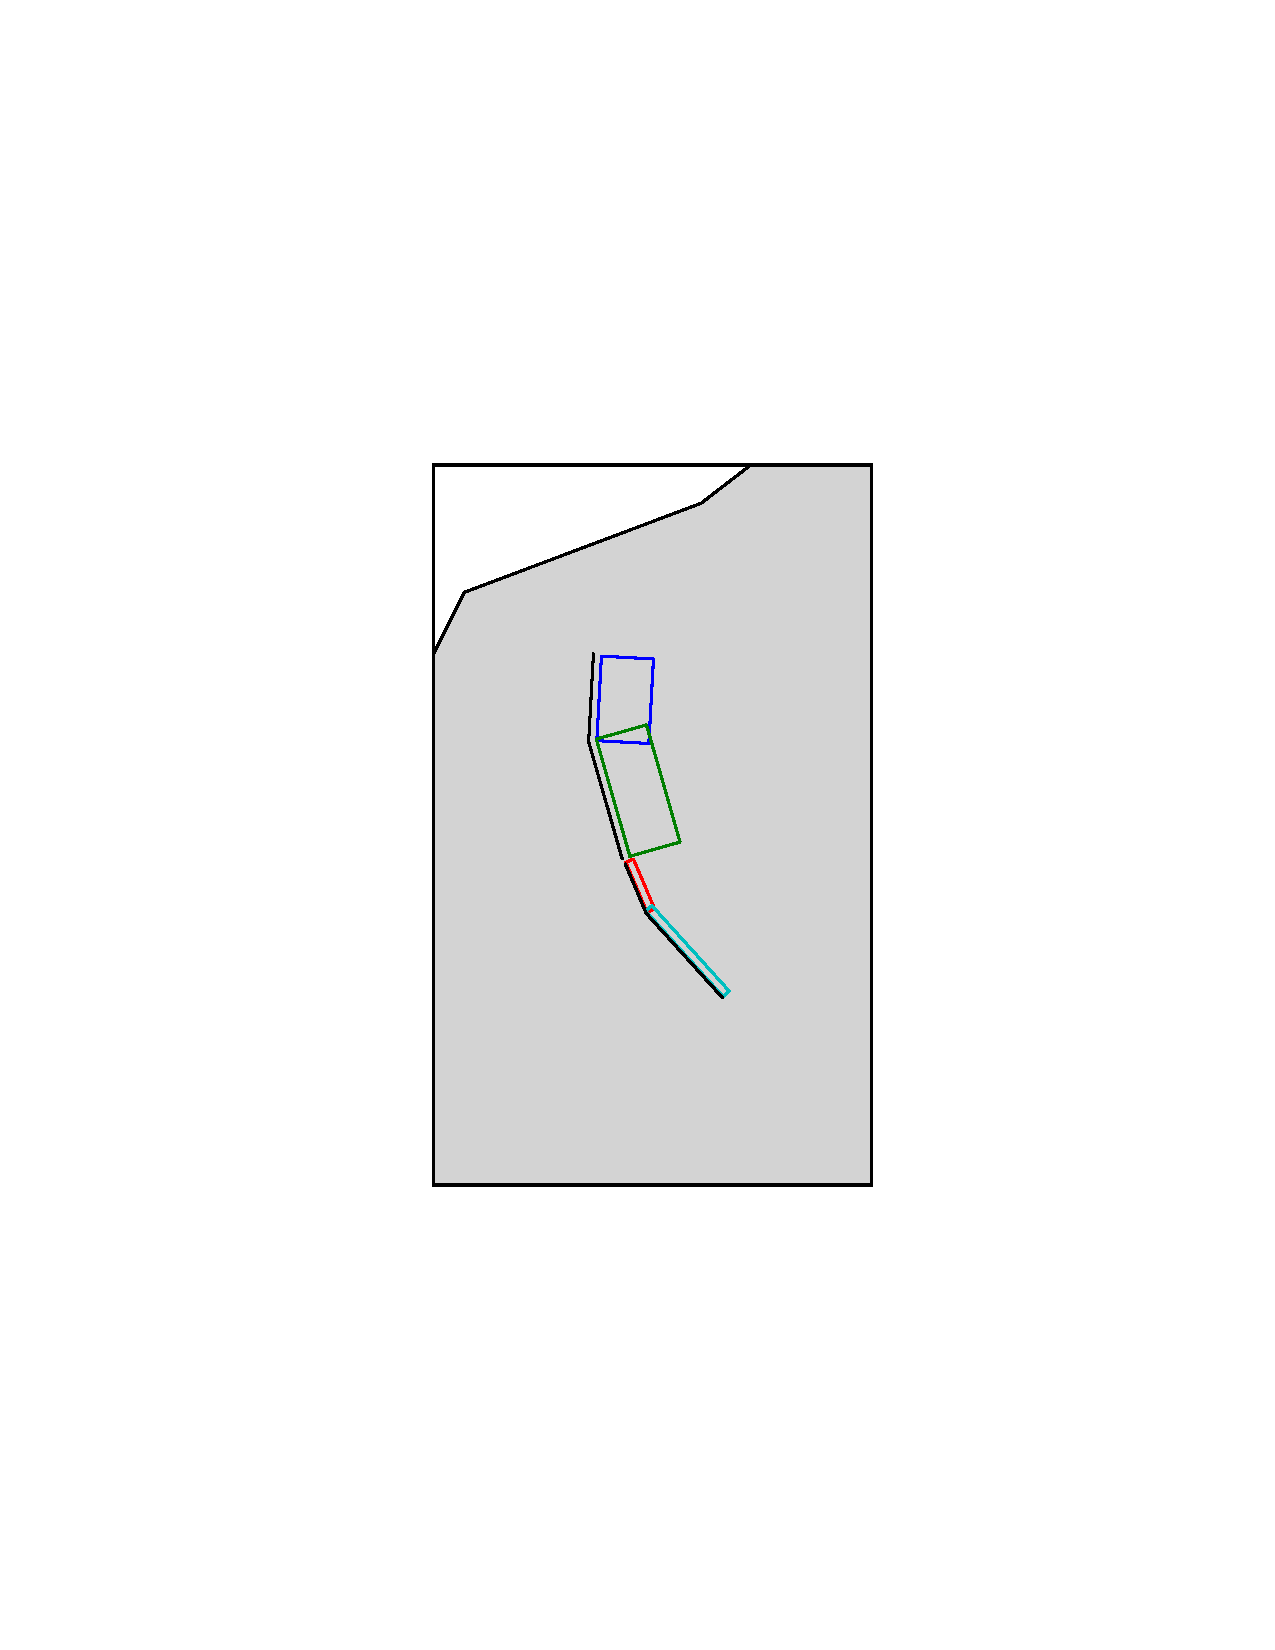
\includegraphics[trim=5cm 7cm 5cm 7cm, clip, width=10cm]{figures/hazard/multi_surface.pdf}
\caption{Geometry of a multi-segmented characteristic fault composed of four
         rectangular ruptures as modelled in OpenQuake.}
\label{fig:char_fault_source}
\end{figure}

\paragraph{Source data}
\begin{itemize}
    \item The characteristic rupture surface is defined through one of the
    following options:
        \begin{itemize}
            \item A list of rectangular ruptures (``planar surfaces'')
            \item A \gls{simplefaultsource} geometry
            \item A \gls{complexfaultsource} geometry
        \end{itemize}
    \item A \gls{frequencymagnitudedistribution}.
    \item Rake angle (specified following the Aki-Richards convention; see
          \citet{aki2002}).
    \item Upper and lower depth values limiting the seismogenic interval.
\end{itemize}

A comprehensive example enumerating the possible rupture surface configurations is shown below. 

\inputminted[firstline=1,firstnumber=1,fontsize=\footnotesize,frame=single,linenos,bgcolor=lightgray]{xml}{oqum/hazard/verbatim/input_characteristic_fault_simple.xml}
\captionof{listing}{Example characteristic fault with simple fault geometry\label{lst:example_characteristic_fault_simple}}

\inputminted[firstline=1,firstnumber=1,fontsize=\footnotesize,frame=single,linenos,bgcolor=lightgray]{xml}{oqum/hazard/verbatim/input_characteristic_fault_complex.xml}
\captionof{listing}{Example characteristic fault with complex fault geometry\label{lst:example_characteristic_fault_complex}}

\inputminted[firstline=1,firstnumber=1,fontsize=\footnotesize,frame=single,linenos,bgcolor=lightgray]{xml}{oqum/hazard/verbatim/input_characteristic_fault_planar.xml}
\captionof{listing}{Example characteristic fault with planar/multi-planar fault geometry\label{lst:example_characteristic_fault_planar}}



%\begin{mdframed}[]
%\inputminted[firstline=1,firstnumber=1,fontsize=%\footnotesize,frame=single,linenos,bgcolor=lightgray]{xml}{oqum/hazard/verbatim/input_nonparametric_source.xml}
%\caption{Example non-parametric source with planar, multi-planar, simple fault %and complex fault geometry}
%\label{lst:example_nonparametric_source}
%\end{mdframed}
%\begin{Verbatim}[frame=single, commandchars=\\\{\}, fontsize=\footnotesize,
    numbers=left, numbersep=2pt]
<?xml version="1.0" encoding="utf-8"?>
<nrml
xmlns="http://openquake.org/xmlns/nrml/0.5"
xmlns:gml="http://www.opengis.net/gml"
>
    <sourceModel name="Test Source Model">
        <nonParametricSeismicSource id="1"
        name="A Non Parametric Source" tectonicRegion="Some TRT">
            <singlePlaneRupture probs_occur="0.544 0.456">
\textcolor{blue}{               <magnitude>8.3</magnitude>}
\textcolor{blue}{               <rake>90.0</rake>}
\textcolor{red}{               <hypocenter depth="26.101" lat="40.726" lon="143.0"/>}
\textcolor{red}{               <planarSurface>}
\textcolor{red}{                   <topLeft depth="9.0" lat="41.6" lon="143.1"/>}
\textcolor{red}{                   <topRight depth="9.0" lat="40.2" lon="143.91"/>}
\textcolor{red}{                   <bottomLeft depth="43.202" lat="41.252" lon="142.07"/>}
\textcolor{red}{                   <bottomRight depth="43.202" lat="39.852" lon="142.91"/>}
\textcolor{red}{               </planarSurface>}
           </singlePlaneRupture>
          <multiPlanesRupture probs_occur="0.9244 0.0756">
\textcolor{blue}{               <magnitude>6.9</magnitude>}
\textcolor{blue}{               <rake>0.0</rake>}
\textcolor{red}{               <hypocenter depth="7.1423" lat="35.296" lon="139.31"/>}
\textcolor{red}{               <planarSurface>}
\textcolor{red}{                   <topLeft depth="2.0" lat="35.363" lon="139.16"/>}
\textcolor{red}{                   <topRight depth="2.0" lat="35.394" lon="138.99"/>}
\textcolor{red}{                   <bottomLeft depth="14.728" lat="35.475" lon="139.19"/>}
\textcolor{red}{                   <bottomRight depth="14.728" lat="35.505" lon="139.02"/>}
\textcolor{red}{               </planarSurface>}
\textcolor{red}{               <planarSurface>}
\textcolor{red}{                   <topLeft depth="2.0" lat="35.169" lon="139.34"/>}
\textcolor{red}{                   <topRight depth="2.0" lat="35.358" lon="139.17"/>}
\textcolor{red}{                   <bottomLeft depth="12.285" lat="35.234" lon="139.45"/>}
\textcolor{red}{                   <bottomRight depth="12.285" lat="35.423" lon="139.28"/>}
\textcolor{red}{               </planarSurface>}
           </multiPlanesRupture>
           <simpleFaultRupture probs_occur="0.157 0.843">
\textcolor{blue}{               <magnitude>7.8</magnitude>}
\textcolor{blue}{               <rake>90.0</rake>}
\textcolor{red}{               <hypocenter depth="22.341" lat="43.624" lon="147.94"/>}
\textcolor{red}{               <simpleFaultGeometry>}
\textcolor{red}{                   <gml:LineString>}
\textcolor{red}{                       <gml:posList>}
\textcolor{red}{                           147.96 43.202}
\textcolor{red}{                           148.38 43.438}
\textcolor{red}{                           148.51 43.507}
\textcolor{red}{                           148.68 43.603}
\textcolor{red}{                           148.76 43.640}
\textcolor{red}{                       </gml:posList>}
\textcolor{red}{                   </gml:LineString>}
\textcolor{red}{                   <dip>30.0</dip>}
\textcolor{red}{                   <upperSeismoDepth>14.5</upperSeismoDepth>}
\textcolor{red}{                   <lowerSeismoDepth>35.5</lowerSeismoDepth>}
\textcolor{red}{               </simpleFaultGeometry>}
           </simpleFaultRupture>
           <complexFaultRupture probs_occur="0.157 0.843">
\textcolor{blue}{               <magnitude>7.8</magnitude>}
\textcolor{blue}{               <rake>90.0</rake>}
\textcolor{red}{               <hypocenter depth="22.341" lat="43.624" lon="147.94"/>}
\textcolor{red}{               <complexFaultGeometry>}
\textcolor{red}{                   <faultTopEdge>}
\textcolor{red}{                       <gml:LineString>}
\textcolor{red}{                           <gml:posList>}
\textcolor{red}{                               148.76 43.64 5.0}
\textcolor{red}{                               148.68 43.603 5.0}
\textcolor{red}{                               148.51 43.507 5.0}
\textcolor{red}{                               148.38 43.438 5.0}
\textcolor{red}{                               147.96 43.202 5.0}
\textcolor{red}{                           </gml:posList>}
\textcolor{red}{                       </gml:LineString>}
\textcolor{red}{                   </faultTopEdge>}
\textcolor{red}{                   <faultBottomEdge>}
\textcolor{red}{                      <gml:LineString>}
\textcolor{red}{                           <gml:posList>}
\textcolor{red}{                               147.92 44.002 35.5}
\textcolor{red}{                               147.81 43.946 35.5}
\textcolor{red}{                               147.71 43.897 35.5}
\textcolor{red}{                               147.5 43.803 35.5}
\textcolor{red}{                               147.36 43.727 35.5}
\textcolor{red}{                           </gml:posList>}
\textcolor{red}{                       </gml:LineString>}
\textcolor{red}{                   </faultBottomEdge>}
\textcolor{red}{               </complexFaultGeometry>}
            </complexFaultRupture>
        </nonParametricSeismicSource>
    </sourceModel>
</nrml>
\end{Verbatim}




\subsection{Non-Parametric Sources}
\subsubsection{Non-Parametric Fault}
\label{desc_nonparametric_fault}
\index{Source type!fault!nonparametric}
\index{Non-Parametric fault|see{Source type}}

The non-parametric fault typology requires that the user indicates the rupture properties (rupture surface, magnitude, rake and hypocentre) and the corresponding probabilities of the rupture. The probabilities are given as a list of floating point values that correspond to the probabilities of $0, 1, 2, \ldots ... N$ occurrences of the rupture within the specified investigation time. Note that there is not, at present, any internal check to ensure that the investigation time to which the probabilities refer corresponds to that specified in the configuration file. As the surface of the rupture is set explicitly, no rupture floating occurs, and, as in the case of the characteristic fault source, the rupture surface can be defined as either a single planar rupture, a list of planar ruptures, a \gls{simplefaultsource} geometry, a \gls{complexfaultsource} geometry, or a combination of different geometries.

Comprehensive examples enumerating the possible configurations are shown below:

\inputminted[firstline=1,firstnumber=1,fontsize=\footnotesize,frame=single,linenos,bgcolor=lightgray]{xml}{oqum/hazard/verbatim/input_nonparametric_planar.xml}
\captionof{listing}{Example non-parametric fault with planar and multi-planar fault geometry\label{lst:example_nonparametric_planar}}
\inputminted[firstline=1,firstnumber=1,fontsize=\footnotesize,frame=single,linenos,bgcolor=lightgray]{xml}{oqum/hazard/verbatim/input_nonparametric_simple.xml}
\captionof{listing}{Example characteristic fault with simple fault geometry\label{lst:example_nonparametric_simple}}
\inputminted[firstline=1,firstnumber=1,fontsize=\footnotesize,frame=single,linenos,bgcolor=lightgray]{xml}{oqum/hazard/verbatim/input_nonparametric_complex.xml}
\captionof{listing}{Example characteristic fault with complex fault geometry\label{lst:example_nonparametric_complex}}

